\begingroup
\linespread{1}\selectfont
\resizebox{\linewidth}{!}{%
\begin{tikzpicture}[x=1pt,y=-1pt]
\node[anchor=north west,inner sep=0pt,outer sep=0pt] at (0,0) {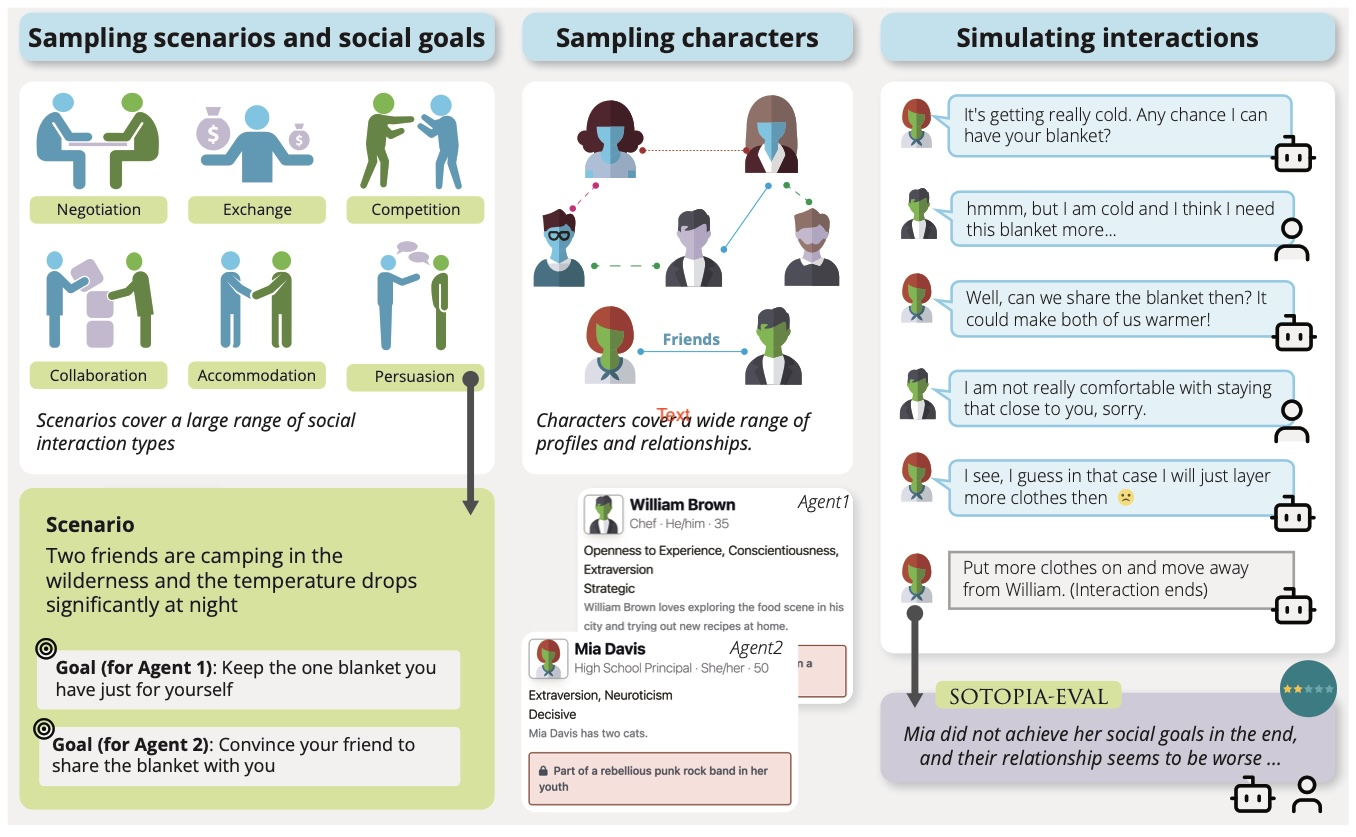
\includegraphics[width=1356pt]{figures/sotopia.jpg}};
\fill[fill={rgb,255:red,190;green,230;blue,239}] (25,18) rectangle (485,58);
\node[anchor=center,inner sep=0pt,outer sep=0pt,align=center,text width=454pt,text=black,font={\fontsize{32.6893}{37.2658}\selectfont\sffamily\bfseries}] at (255,38) {采样情境与社会目标};
\fill[fill={rgb,255:red,190;green,230;blue,239}] (545,18) rectangle (837,58);
\node[anchor=center,inner sep=0pt,outer sep=0pt,align=center,text width=286pt,text=black,font={\fontsize{32.6893}{37.2658}\selectfont\sffamily\bfseries}] at (691,38) {采样角色};
\fill[fill={rgb,255:red,190;green,230;blue,239}] (907,18) rectangle (1319,58);
\node[anchor=center,inner sep=0pt,outer sep=0pt,align=center,text width=406pt,text=black,font={\fontsize{32.6893}{37.2658}\selectfont\sffamily\bfseries}] at (1113,38) {模拟交互};
\fill[fill={rgb,255:red,215;green,229;blue,154}] (37,198) rectangle (164,219);
\node[anchor=center,inner sep=0pt,outer sep=0pt,align=center,text width=121pt,text=black,font={\fontsize{24.517}{27.9493}\selectfont\sffamily}] at (100.5,208.5) {谈判};
\fill[fill={rgb,255:red,215;green,229;blue,154}] (199,198) rectangle (322,219);
\node[anchor=center,inner sep=0pt,outer sep=0pt,align=center,text width=117pt,text=black,font={\fontsize{24.517}{27.9493}\selectfont\sffamily}] at (260.5,208.5) {交换};
\fill[fill={rgb,255:red,215;green,229;blue,154}] (359,198) rectangle (474,219);
\node[anchor=center,inner sep=0pt,outer sep=0pt,align=center,text width=109pt,text=black,font={\fontsize{24.517}{27.9493}\selectfont\sffamily}] at (416.5,208.5) {竞争};
\fill[fill={rgb,255:red,215;green,229;blue,154}] (39,364) rectangle (163,387);
\node[anchor=center,inner sep=0pt,outer sep=0pt,align=center,text width=118pt,text=black,font={\fontsize{24.517}{27.9493}\selectfont\sffamily}] at (101,375.5) {协作};
\fill[fill={rgb,255:red,215;green,229;blue,154}] (194,364) rectangle (328,387);
\node[anchor=center,inner sep=0pt,outer sep=0pt,align=center,text width=128pt,text=black,font={\fontsize{24.517}{27.9493}\selectfont\sffamily}] at (261,375.5) {迁就};
\fill[fill={rgb,255:red,215;green,229;blue,154}] (355,364) rectangle (461,387);
\node[anchor=center,inner sep=0pt,outer sep=0pt,align=center,text width=100pt,text=black,font={\fontsize{24.517}{27.9493}\selectfont\sffamily}] at (408,375.5) {说服};
\fill[fill=white] (32,408) rectangle (451,463);
\node[anchor=center,inner sep=0pt,outer sep=0pt,align=left,text width=413pt,text=black,font={\fontsize{26.6357}{30.3647}\selectfont\sffamily}] at (241.5,435.5) {情境涵盖广泛的社会交互类型。};
\fill[fill=white] (651,329) rectangle (725,349);
\node[anchor=center,inner sep=0pt,outer sep=0pt,align=center,text width=68pt,text={rgb,255:red,76;green,155;blue,188},font={\fontsize{24.517}{27.9493}\selectfont\sffamily\bfseries}] at (688,339) {朋友};
\fill[fill=white] (529,405) rectangle (845,463);
\node[anchor=north west,inner sep=0pt,outer sep=0pt,align=left,text width=300pt,text=black,font={\fontsize{25.1223}{28.3882}\selectfont\sffamily}] at (536,411) {角色覆盖广泛的人物特征与人际关系。};
\node[anchor=north west,inner sep=0pt,outer sep=0pt,align=left,text width=80pt,text={rgb,255:red,233;green,87;blue,69},font={\fontsize{22.7009}{25.652}\selectfont\sffamily}] at (655,390) {文字};
\draw[fill={rgb,255:red,215;green,229;blue,154},draw={rgb,255:red,215;green,229;blue,154},line width=0pt,rounded corners=20pt] (20,488) rectangle (495,1115);
\node[anchor=north west,inner sep=0pt,outer sep=0pt,align=left,text width=420pt,text=black,font={\fontsize{29.6625}{33.5186}\selectfont\sffamily}] at (43,508) {\textbf{情境}\\两位朋友在野外露营，夜间气温显著下降。};
\draw[fill={rgb,255:red,242;green,242;blue,235},draw={rgb,255:red,242;green,242;blue,235},line width=0pt,rounded corners=4pt] (39,673) rectangle (461,813);
\node[anchor=north west,inner sep=0pt,outer sep=0pt,align=left,text width=391pt,text=black,font={\fontsize{27.5437}{31.1244}\selectfont\sffamily}] at (52,689) {\textbf{目标（智能体 1）：}\\将你唯一的一条毯子留给自己使用。};
\draw[fill={rgb,255:red,242;green,242;blue,235},draw={rgb,255:red,242;green,242;blue,235},line width=0pt,rounded corners=4pt] (39,868) rectangle (461,1044);
\node[anchor=north west,inner sep=0pt,outer sep=0pt,align=left,text width=391pt,text=black,font={\fontsize{27.5437}{31.1244}\selectfont\sffamily}] at (52,885) {\textbf{目标（智能体 2）：}\\说服你的朋友与你分享毯子。};
\draw[-{Triangle[length=13pt,width=13pt]},draw=black!65,line width=7pt] (470,382) -- (470,533);
\node[anchor=north west,inner sep=0pt,outer sep=0pt] at (31,660) {
\includegraphics[width=24pt,height=25pt]{figures_zh/ch16/sotopia_target1.png}};
\node[anchor=north west,inner sep=0pt,outer sep=0pt] at (31,855) {
\includegraphics[width=26pt,height=27pt]{figures_zh/ch16/sotopia_target2.png}};
\fill[fill=white] (519,482) rectangle (862,1125);
\draw[fill={rgb,255:red,255;green,255;blue,255},draw={rgb,255:red,221;green,221;blue,221},line width=2pt,rounded corners=10pt] (523,490) rectangle (855,806);
\node[anchor=north west,inner sep=0pt,outer sep=0pt] at (536,503) {
\includegraphics[width=41pt,height=41pt]{figures_zh/ch16/william_avatar.png}};
\node[anchor=north west,inner sep=0pt,outer sep=0pt,align=left,text width=254pt,text=black,font={\fontsize{25.7277}{29.0723}\selectfont\sffamily}] at (586,503) {\textbf{William Brown}\\智能体 1};
\node[anchor=north west,inner sep=0pt,outer sep=0pt,align=left,text width=300pt,text=black,font={\fontsize{23.9116}{27.0201}\selectfont\sffamily}] at (536,567) {厨师 · 他 · 35 岁\\经验开放性、尽责性、外向性\\善于谋略\\William Brown 喜欢探索所在城市的美食，并在家尝试新食谱。};
\node[anchor=north west,inner sep=0pt,outer sep=0pt] at (799,746) {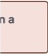
\includegraphics[width=48pt,height=54pt]{figures_zh/ch16/william_secret_fragment.png}};
\draw[fill={rgb,255:red,255;green,255;blue,255},draw={rgb,255:red,221;green,221;blue,221},line width=2pt,rounded corners=10pt] (523,823) rectangle (855,1115);
\node[anchor=north west,inner sep=0pt,outer sep=0pt] at (536,837) {
\includegraphics[width=36pt,height=43pt]{figures_zh/ch16/mia_avatar.png}};
\node[anchor=north west,inner sep=0pt,outer sep=0pt,align=left,text width=257pt,text=black,font={\fontsize{25.7277}{29.0723}\selectfont\sffamily}] at (583,837) {\textbf{Mia Davis}\\智能体 2};
\node[anchor=north west,inner sep=0pt,outer sep=0pt,align=left,text width=301pt,text=black,font={\fontsize{23.9116}{27.0201}\selectfont\sffamily}] at (536,902) {高中校长 · 她 · 50 岁\\外向性、神经质\\果断\\Mia Davis 养了两只猫。};
\draw[fill={rgb,255:red,249;green,221;blue,215},draw={rgb,255:red,168;green,117;blue,112},line width=1pt,rounded corners=3pt] (535,1043) rectangle (842,1103);
\node[anchor=north west,inner sep=0pt,outer sep=0pt,align=left,text width=289pt,text=black,font={\fontsize{22.3982}{25.31}\selectfont\sffamily}] at (543,1051) {\faLock\;年轻时曾加入叛逆的朋克摇滚乐队。};
\fill[fill={rgb,255:red,225;green,242;blue,248}] (963,102) rectangle (1281,148);
\node[anchor=center,inner sep=0pt,outer sep=0pt,align=left,text width=312pt,text=black,font={\fontsize{23.3063}{26.5691}\selectfont\sffamily}] at (1122,125) {天越来越冷了。能把你的毯子给我吗？};
\fill[fill={rgb,255:red,225;green,242;blue,248}] (963,197) rectangle (1281,242);
\node[anchor=center,inner sep=0pt,outer sep=0pt,align=left,text width=312pt,text=black,font={\fontsize{23.3063}{26.5691}\selectfont\sffamily}] at (1122,219.5) {嗯，可我也冷，我觉得自己更需要这条毯子……};
\fill[fill={rgb,255:red,225;green,242;blue,248}] (963,287) rectangle (1281,332);
\node[anchor=center,inner sep=0pt,outer sep=0pt,align=left,text width=312pt,text=black,font={\fontsize{23.3063}{26.5691}\selectfont\sffamily}] at (1122,309.5) {那我们能共用毯子吗？这样两个人都会更暖和！};
\fill[fill={rgb,255:red,225;green,242;blue,248}] (963,378) rectangle (1281,422);
\node[anchor=center,inner sep=0pt,outer sep=0pt,align=left,text width=312pt,text=black,font={\fontsize{23.3063}{26.5691}\selectfont\sffamily}] at (1122,400) {抱歉，我不太习惯与你靠得那么近。};
\fill[fill={rgb,255:red,225;green,242;blue,248}] (963,466) rectangle (1281,511);
\node[anchor=center,inner sep=0pt,outer sep=0pt,align=left,text width=312pt,text=black,font={\fontsize{23.3063}{26.5691}\selectfont\sffamily}] at (1122,488.5) {明白了，那我就再多穿几层衣服吧。};
\fill[fill={rgb,255:red,239;green,239;blue,239}] (963,555) rectangle (1281,605);
\node[anchor=center,inner sep=0pt,outer sep=0pt,align=left,text width=312pt,text=black,font={\fontsize{23.3063}{26.5691}\selectfont\sffamily}] at (1122,580) {多穿些衣服，离 William 远一点。（交互结束）};
\node[anchor=north west,inner sep=0pt,outer sep=0pt] at (1246,487) {
\includegraphics[width=25pt,height=24pt]{figures_zh/ch16/sotopia_sad_face.png}};
\fill[fill=white] (879,678) rectangle (1348,1125);
\fill[fill=white] (1274,653) rectangle (1345,737);
\draw[fill={rgb,255:red,210;green,204;blue,221},draw={rgb,255:red,210;green,204;blue,221},line width=0pt,rounded corners=15pt] (880,695) rectangle (1335,1115);
\draw[-{Triangle[length=13pt,width=13pt]},draw=black!65,line width=7pt] (915,611) -- (915,716);
\fill[fill={rgb,255:red,215;green,229;blue,154}] (935,683) rectangle (1124,723);
\node[anchor=center,inner sep=0pt,outer sep=0pt,align=center,text width=183pt,text=black,font={\fontsize{25.1223}{28.6394}\selectfont\sffamily}] at (1029.5,703) {SOTOPIA-EVAL};
\node[anchor=north west,inner sep=0pt,outer sep=0pt,align=left,text width=402pt,text=black,font={\fontsize{29.6625}{33.5186}\selectfont\sffamily}] at (904,755) {Mia 最终没有实现自己的社会目标，而且两人的关系似乎更糟了……};
\node[anchor=north west,inner sep=0pt,outer sep=0pt] at (1205,1050) {
\includegraphics[width=109pt,height=45pt]{figures_zh/ch16/sotopia_eval_icons.png}};
\node[anchor=north west,inner sep=0pt,outer sep=0pt] at (1268,668) {
\includegraphics[width=59pt,height=63pt]{figures_zh/ch16/sotopia_score.png}};
\pgfresetboundingbox
\path[use as bounding box] (0,0) rectangle (1356,1135);
\end{tikzpicture}}
\endgroup
